\begin{figure}
    \centering
    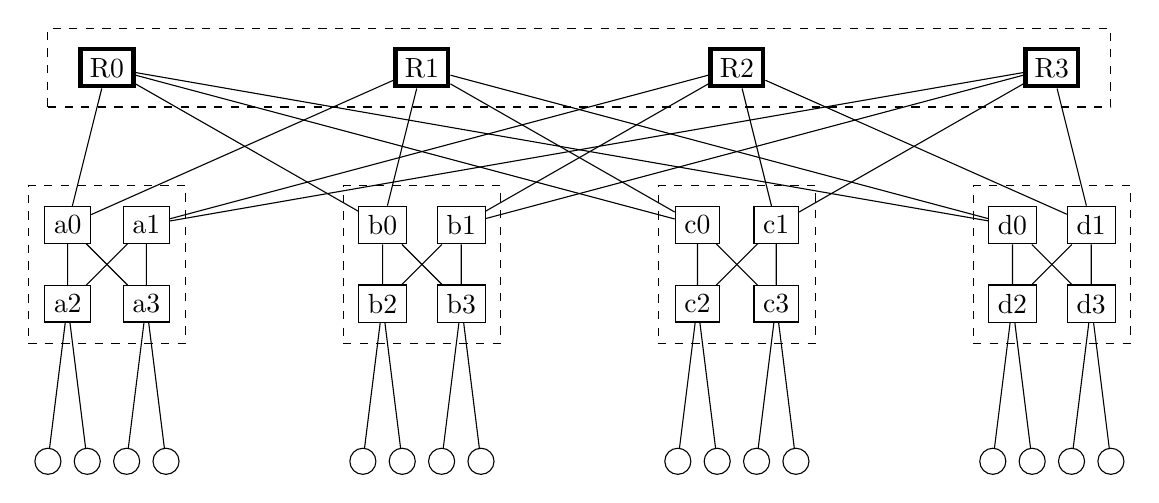
\begin{tikzpicture}[
        nsty/.style={circle,draw,font=\large},
        ssty/.style={font=\LARGE},
        rswsty/.style={rectangle,draw,ultra thick},
        lswsty/.style={rectangle,draw},
        nsty/.style={circle,draw,font=\tiny},
    ]
    \foreach \o/\l in {0/a,4/b,8/c,12/d}{
        \node (b\o) at (\o+0.75, 2.5) [rectangle, draw, dashed,
            minimum width=2cm, minimum height=2cm] {};
        \node (s\o0) at (\o+0.25, 3) [lswsty] {\l0};
        \node (s\o1) at (\o+1.25, 3) [lswsty] {\l1};
        \node (s\o2) at (\o+0.25, 2) [lswsty] {\l2};
        \node (s\o3) at (\o+1.25, 2) [lswsty] {\l3};
        \foreach \x in {0,1,2,3} {
            \node (n\o\x) at (\x/2+\o, 0) [nsty] {};
        }
        \draw (s\o0) -- (s\o2) -- (n\o0);
        \draw (s\o0) -- (s\o3) -- (n\o2);
        \draw (s\o1) -- (s\o2) -- (n\o1);
        \draw (s\o1) -- (s\o3) -- (n\o3);
    }
    \node (r0) at (0.75,5) [rswsty] {R0};
    \node (r1) at (4.75,5) [rswsty] {R1};
    \node (r2) at (8.75,5) [rswsty] {R2};
    \node (r3) at (12.75,5) [rswsty] {R3};
    \node () at (6.75, 5) [rectangle, draw, dashed,
            minimum width=13.5cm, minimum height=1cm] {};
    \foreach \i in {0,4,8,12}{
        
        \draw[] (r0) -- (s\i0);
        \draw[] (r1) -- (s\i0);
        \draw[] (r2) -- (s\i1);
        \draw[] (r3) -- (s\i1);
    }
    \end{tikzpicture}
	\caption[Sixteen-Node Two-Level Fat Tree Network]{
        Sample non-blocking fat-tree network connecting 16 nodes.
        The network uses 4-port switches, but combines them into groups to create leaf/root switches.
        The top row of switches encompass the root of the network, and the groups of four switches in the middle are the leaf switches. 
     }
	\label{fig:fat-tree-topology}
\end{figure}
